\documentclass{article}

\usepackage{exercises}
\withsolutions

\begin{document}
\sheet[20202]{Zweittermin}
\begin{exercise}{Depth-first search}
  Betrachten Sie einen Aufruf der in der Vorlesung vorgestellten Tiefensuche (Pseudocode siehe Algorithmen 1 \& 2) auf dem gerichteten Graphen $G = (V, E)$ aus Abbildung 1. Nehmen Sie an, dass alle Adjazenzlisten lexikographisch sortiert sind \& for-Schleifen über alle Knoten diese auch in lexikographischer Reihenfolge betrachten.
  \begin{algorithm}[ht]
    \caption{DFS($G$)}
    \KwData{$G = (V, E)$}
    \KwResult{Knoteneigenschaften $d(u), f(u), \pi(u)$ für alle $u \in V$}
    \For{$u \in V$}{
      \If{$\text{color}(u) = \text{white}$}{
        $\text{DFS-VISIT}(u)$
      }
    }
  \end{algorithm}

  \begin{algorithm}[ht]
    \caption{DFS-VISIT($G, u$)}
    \KwData{$G = (V, E)$, $u \in V$}
    \KwResult{Knoteneigenschaften $d(u), f(u), \pi(u)$}
    $\text{color}(u) \gets \text{gray}$ \\
    $time \gets time + 1$ \\
    $d(u) \gets time$ \\
    \For{$v \in \text{Adj}(u)$}{
      \If{$\text{color}(v) = \text{white}$}{
        $\pi(v) \gets u$ \\
        $\text{DFS-VISIT}(v)$
      }
    }
    $\text{color}(u) \gets \text{black}$ \\
    $time \gets time + 1$ \\
    $f(u) \gets time$
  \end{algorithm}

  \begin{figure}[ht]
    \centering
    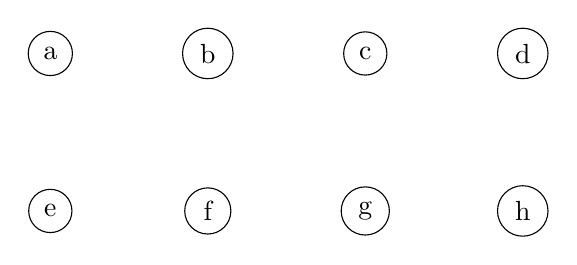
\begin{tikzpicture}
      \node[draw, circle] (a) at (0, 0) {a};
      \node[draw, circle] (b) at (2, 0) {b};
      \node[draw, circle] (c) at (4, 0) {c};
      \node[draw, circle] (d) at (6, 0) {d};
      \node[draw, circle] (e) at (0, -2) {e};
      \node[draw, circle] (f) at (2, -2) {f};
      \node[draw, circle] (g) at (4, -2) {g};
      \node[draw, circle] (h) at (6, -2) {h};
      % TODO: draw graph
    \end{tikzpicture}
    \caption{Gerichteter Graph $G$}
  \end{figure}

  Zeichnen Sie den entstehenden Tiefensuchwald. Geben Sie außerdem für alle Knoten $u \in V$ die berechneten Knoteneigenschaften $d(u)$ \& $f(u)$ am Ende des Algorithmus an.
\end{exercise}

\setcounter{subsection}{2}
\begin{eexercises}{Hashing}{
    Es seien die Hashfunktionen $h_1$ \& $h_2$ wie folgt definiert:
    \begin{align*}
      h_1(x) & = (3x + 5) \mod 7 \\
      h_2(x) & = (4x + 6) \mod 8
    \end{align*}
  }
  \item Illustrieren Sie die Hashatabelle der Größe 7, die entsteht, wenn zur Einfügung aller Elemente aus $K = \{1, 2, 4, 16, 20, 23, 26\}$ nacheinander in der angegebene Reihenfolge mit Hilfe von $h_1$ eingefügt werden.
  \item Illustrieren Sie die Hashatabelle der Größe 8, die entsteht, wenn zur Einfügung aller Elemente aus $K = \{1, 2, 4, 16, 20, 23, 26\}$ nacheinander in der angegebene Reihenfolge mit Hilfe von $h_2$ eingefügt werden
  \item Geben Sie jeweils für $h_1$ \& $h_2$ an, ob es sich um eine gute Wahl zur Konstruktion einer Hashtabelle mittels geschlossener Adressierung handelt oder nicht. Begründen Sie Ihre Aussage.
\end{eexercises}

\begin{eexercises}{O-Notation}{
  Jede der folgenden Teilaufgaben spezifiziert zwei Funktionen $f(n)$ \& $g(n)$. Bestimmen Sie jeweils, ob die vier Relationen $f(n) = \mathcal{O}(g(n)), f(n) = \mathcal{O}(g(n)), f(n) = \Omega(g(n)), f(n) = \omega(g(n))$ gelten (es sind also pro Teilaufgabe vier Antworten zu geben). Beweisen Sie Ihre Antwort jeweils kurz. Nutzen Sie dazu die Eigenschaften der asymptotischen Landau-Notation aus der Vorlesung (wie z.B. die ursprüngliche Definition, die Charakterisierung über Grenzwerte oder die darauffolgenden Lemmata).
    \hint{Die Basis des Logarithmus ist 2.}
    }
    \item $f(n) = 2n^2 + 23n^{3/2} + \log{n} -42$ und $g(n) = n^{2.001}$
    \item $f(n) = n \cdot (1 + (-1)^n)$ und $g(n) = 2n$
    \item $f(n) = 2\sqrt{n}$ und $g(n) = (3/2)^n$
    \item $f(n) = \sum_{i=1}^n \log{i}$ und $g(n) = n \log{n}$
\end{eexercises}

\begin{eexercises}{Algorithmenentwurf}{
    Gegeben sei ein ungerichteter, zusammenhängender Graph $G = (V, E)$. Ein Knoten $u \in V$ heißt Nadelöhr, wenn der Graph $G - u = (V \setminus \{u\}, E \setminus \{(v, w) \in E | v = u \lor w = u\})$ unzusammenhängend ist. Abbildung 2 zeigt ein Beispiel eines Graphen mit Nadelöhr.
  }
  \item Beschreiben Sie einen Algorithmus (als Pseudocode oder in Textform), der bei Eingabe eines ungerichteten, zusammenhängenden Graphen $G$ in Adjazenzlistendarstellung bestimmt, ob $G$ ein Nadelöhr besitzt. Ihr Algorithmus sollte Laufzeit $\bigO(|V| + |V| \cdot |E|)$ haben.
  \item Analysieren Sie die Laufzeit Ihres Algorithmus.
  \item Beweisen Sie die Korrektheit Ihres Algorithmus.
\end{eexercises}

\begin{eexercises}{Algorithmenentwurf II}{
    Entwerfen Sie anhand der folgenden Arbeitsschritte einen Divide \& Conquer Algorithmus, der bei Eingabe zweier natürlicher Zahlen $x \in \mathbb{N}$ und $n \in \mathbb{N}$ die Potenz
    \begin{equation*}
      x^n = x \cdot x \cdot \ldots \cdot x
    \end{equation*}
    in Laufzeit $\bigO(\log n)$ berechnet. Als arithmetische Operationen mit konstanter Laufzeit sind dabei lediglich die Addition, Subtraktion sowie Multiplikation zweier ganzer Zahlen erlaubt. Auch die Abfrage ob eine Zahl gerade oder ungerade ist, kann in konstanter Laufzeit erfolgen.
  }
  \item Beschreiben Sie Ihre algorithmische Idee zunächst informell.
  \hint{Überlegen Sie sich eine rekursive Formulierung für $x^n$ und erklären Sie, wie Ihr Algorithmus diese nutzt. Achten Sie darauf, dass die rekursive Formulierung die geforderte Laufzeitschranke ermöglicht.}
  \item Formulieren Sie Ihren Algorithmus in Pseudocode.
  \item Geben Sie die Laufzeit Ihres Algorithmus als Rekursionsgleichung an.
  \item Analysieren Sie die Laufzeit Ihres Algorithmus möglichst genau in der $\bigO$-Notation mit Hilfe der Substitutionsmethode. Sie können dabei annehmen, dass $n$ eine Zweierpotenz ist. Sollten Sie keine Lösung zu 3. haben, dürfen Sie stattdessen die Rekursionsgleichung $T(n) = 3 \cdot T(n/3) + 42$ mit $T(1) = 23$ auflösen.
  \hint{Ein Induktionsbeweis der Laufzeit ist nicht notwendig, aber aus Ihrer Rechnung muss klar hervorgehen, wie Sie zu Ihrer Lösung kommen.}
\end{eexercises}

\begin{eexercises}{Dynamische Programmierung}{
    Das Unternehmen Alset möchte aus $n$ verschiedenen Prototypen eines neuen elektrischen Traktors eine möglichst große Teilmenge realisieren. Die Realisierung von Protoyp $i$ verursacht Kosten $c_i \in \mathbb{N}$. Zur Umsetzung der ausgewählten Prototypen steht ein Budget $B \in \mathbb{N}$ zur Verfügung, welches die Kosten aller ausgewählten Prototypen decken muss.
  }
  \item Sei $\text{OPT}(i, b)$ die maximale Anzahl der ersten $i \in \{0, 1, \ldots, n\}$ Prototypen, die mit dem Budget $b \in \{0, 1, \ldots, B\}$ realisierbar sind. Finden Sie eine rekursive Formulierung für $\text{OPT}(i, b)$ und begründen Sie kurz deren Korrektheit.
  \hint{Nutzen Sie zur Lösung dieser Teilaufgabe ein aus der Vorlesung bekanntes Problem, welches die obige Situation modelliert.}
  \item Zur Realisierung von Prototyp $i$ müssen nun zusätzlich $m_i \in \mathbb{N}$ Mitarbeiter bereitgestellt werden. Es stehen insgesamt $M \in \mathbb{N}$, von denen jeder bei der Umsetzung von höchstens einem (beliebigen) Prototypen helfen kann. Entwickeln Sie eine rekursive Formulierung für die maximale Anzahl realisierbarer Projekte unter diesen zusätzlichen Randbedingungen \& begründen Sie kurz deren Korrektheit. Beachten Sie dabei die Laufzeitanforderung aus 3.
  \item Beschreiben Sie in Pseudocode einen Algorithmus, der mittels dynamischer Programmierung in Zeit $\bigO(n \cdot B \cdot M)$ die maximale Anzahl realisierbarer Projekte, unter Berücksichtigung des Gesamtbudgets und der verfügbaren Mitarbeiter, bestimmt. Die konkrete Teilmenge der zugehörigen Prototypen muss nicht bestimmt werden. Als Eingabe erhält Ihr Algorithmus die Werte $B$ und $M$ sowie die $n$-elementigen Arrays $c = [c_1, \ldots, c_n]$ und $m = [m_1, \ldots, m_n]$.
\end{eexercises}

\begin{eexercises}{Algorithmenentwurf III}{
    Um den Netzausbau in Deutschland voran zu treiben, hat sich der Telekommunikationsanbieter Mokelet dazu entschlossen, jedes Haus in dem Dorf Hintertupfingen mit 5G-Empfang zu versorgen. In Hintertupfingen gibt es genau $n \in \mathbb{N}$ Häuser, die alle entlang einer schnurgeraden, $k \in \mathbb{N}$ Kilometer langen Straße stehen. Um ein Haus mit 5G-Empfang zu versorgen, muss Mokelet 5G-Masten entlang der Straße aufstellen. Ein einzelner 5G-Mast kann beliebig viele Häuser in einer Entfernung bis zu 3 Kilometer versorgen. Da Hintertupfingen nur spärlich besiedelt ist, muss Mokelet genau planen, wo die teuren 5G-Masten errichtet werden sollen.\par
    Wir modellieren die Straße als Strecke auf dem Zahlenstrahl zwischen 0 und $k$. Der Standort des $i$-ten Hauses kann als (rationale) Zahl $h_i \in [0, k]$ beschrieben werden. Masten können an beliebigen (rationalen) Punkten im Intervall $[0, k]$ errichtet werden.
    \hint{Die Lösung einer Strategie $A$, die 5G-Masten aufstellt, kann zum Beispiel als Folge von rationalen Zahlen $a_1 < a_2$ beschrieben mit $a_2 \in [0, k]$ beschreiben werden. Der $i$-te 5G-Mast wird dabei an Position $a_i$ errichtet.}
  }
  \item Wo wäre (im Hinblick auf eine optimale Lösung) ein geeigneter Standort für die 5G-Mast, der das erste ("am weitesten links liegende") Haus versorgt?
  \item Beschreiben Sie einen Greedy-Algorithmus, der bei Eingabe eines Arrays $H = [h_1, \ldots h_n]$ der $n$ Haus-Standorte (in aufsteigender Reihenfolge) und der Länge $k$ der Straße in Laufzeit $\bigO(n)$ die minimale Anzahl an 5G-Masten bestimmt, die zur vollständigen Versorgung von Hintertupfingen notwendig sind.
  \item Analysieren Sie die Laufzeit Ihres Algorithmus.
  \item Beweisen Sie, dass Ihr Algorithmus eine optimale Lösung liefert.
\end{eexercises}
\end{document}